\documentclass{standalone}
\usepackage{tikz}
\usetikzlibrary{arrows,decorations.markings,calc,positioning}
\begin{document}
\begin{tikzpicture}[font=\scriptsize]

   % top row
   \begin{scope}[shift={(-1.5,0.0)}]
      \fill[black!2] (0,0) rectangle (17.9,-3.4);
      \node[inner sep=0cm] at ( 3.0,-1.45) {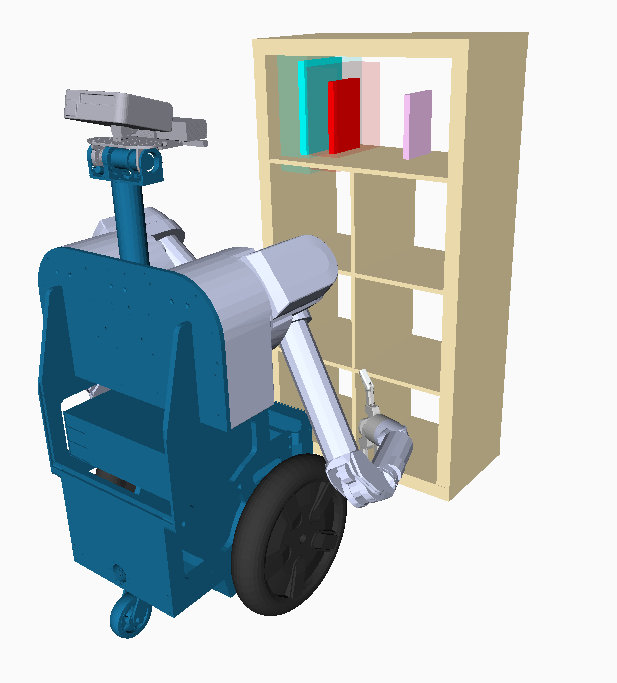
\includegraphics[width=2.6cm]{figs/herbarm-traj0-t000.png}};
      \node[inner sep=0cm] at ( 5.7,-1.45) {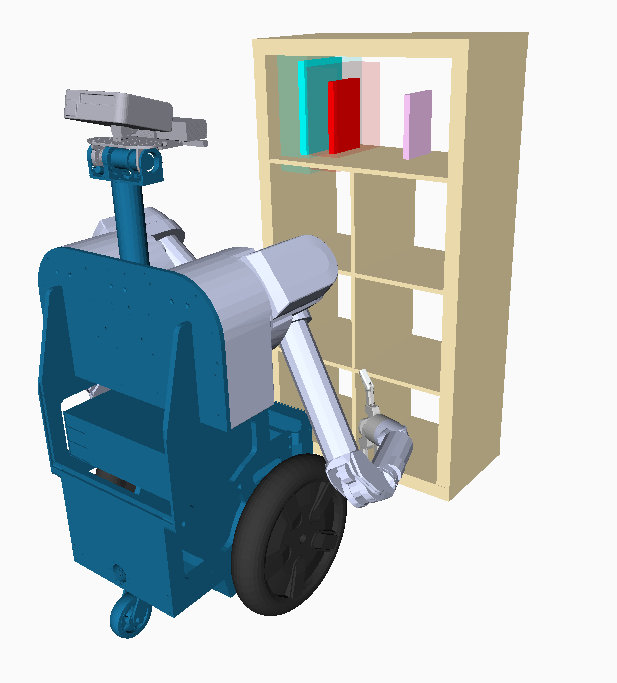
\includegraphics[width=2.6cm]{figs/herbarm-traj0-t000.png}};
      \node[inner sep=0cm] at ( 8.4,-1.45) {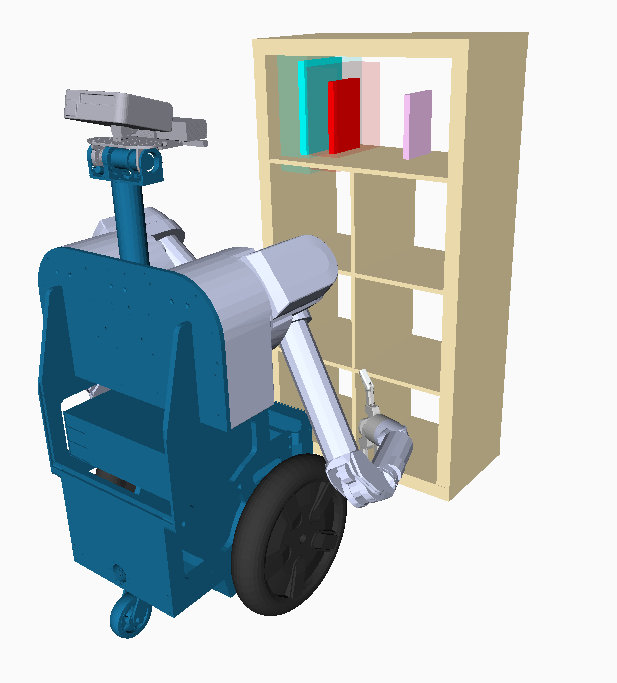
\includegraphics[width=2.6cm]{figs/herbarm-traj0-t000.png}};
      \node[inner sep=0cm] at (11.1,-1.45) {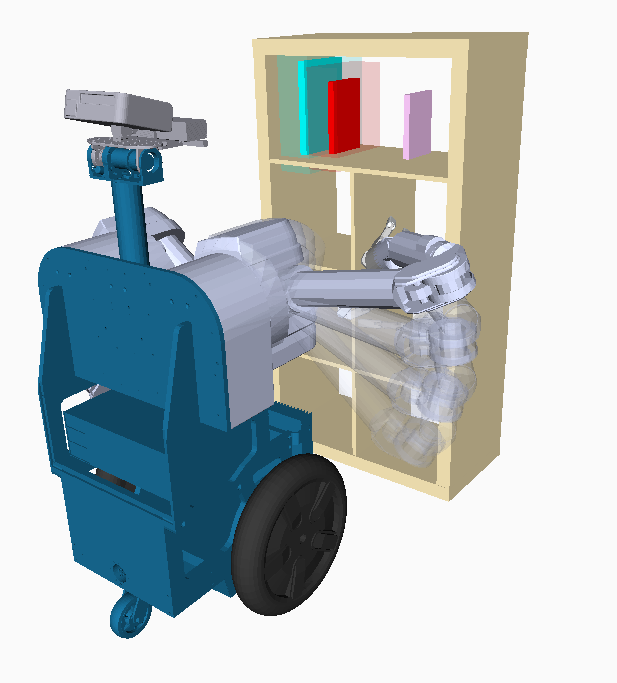
\includegraphics[width=2.6cm]{figs/herbarm-traj0-t007.png}};
      \node[inner sep=0cm] at (13.8,-1.45) {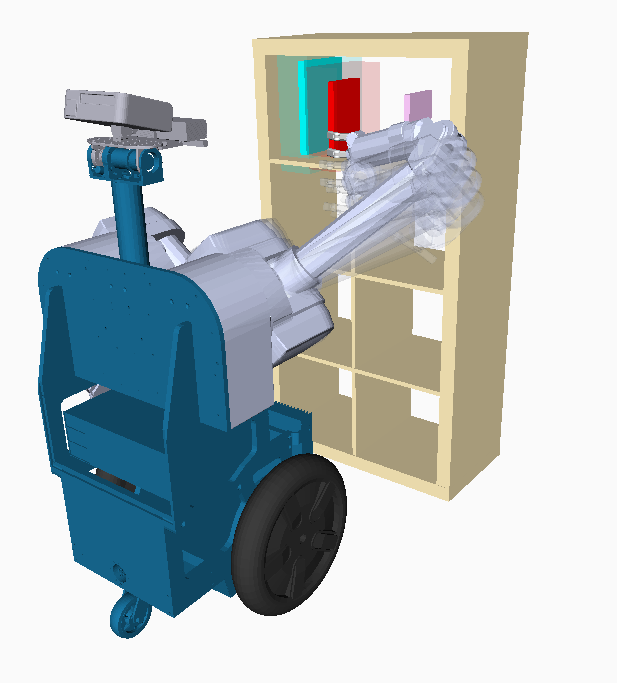
\includegraphics[width=2.6cm]{figs/herbarm-traj0-t016.png}};
      \node[inner sep=0cm] at (16.5,-1.45) {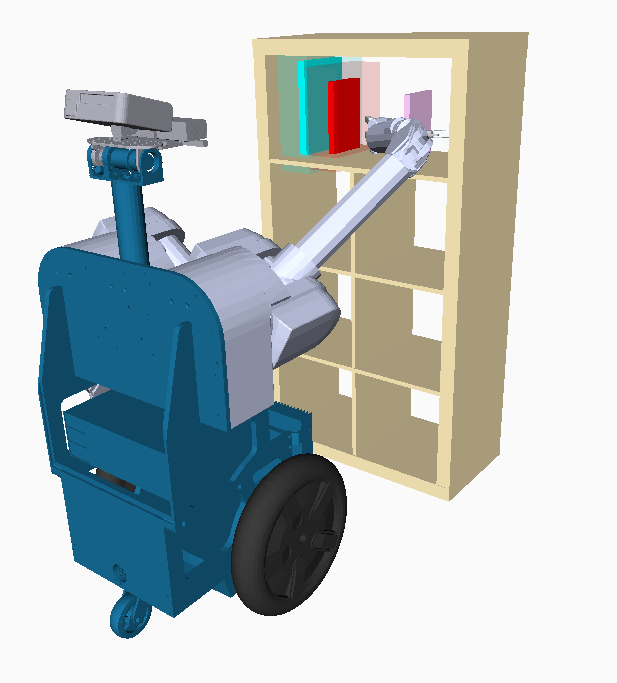
\includegraphics[width=2.6cm]{figs/herbarm-traj0-t026.png}};
      \node[fill=black!10,inner sep=0pt,minimum height=0.4cm,minimum width=5.54cm] at (4.47,-3.1) {Planning: 2.80s};
      \node[fill=black!10,inner sep=0pt,minimum height=0.4cm,minimum width=10.46cm] at (12.57,-3.1) {Execution: 5.29s};
      \node at (0.85,-2.2) {$\lambda_p = 0.0$};
      \draw[black!5] (0,0) rectangle (17.9,-3.4);
   \end{scope}
   
   % middle row
   \begin{scope}[shift={(-1.5,-3.6)}]
      \fill[black!2] (0,0) rectangle (17.9,-3.4);
      \node[inner sep=0cm] at ( 3.0,-1.45) {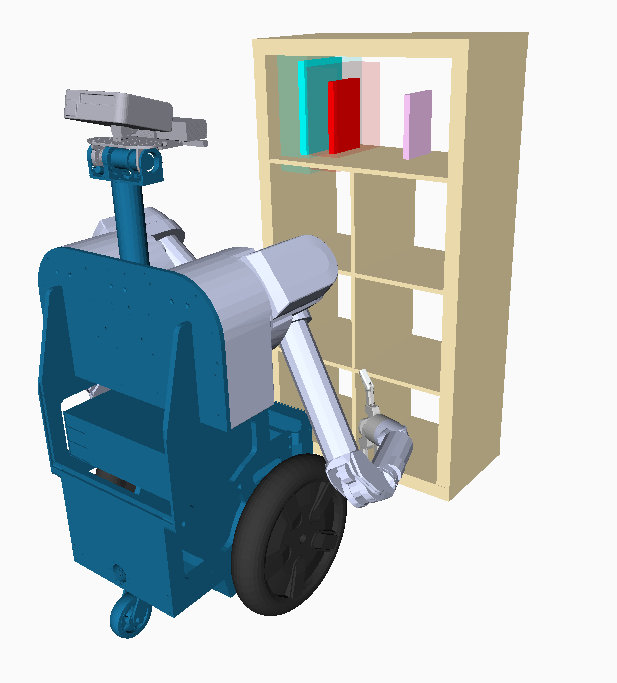
\includegraphics[width=2.6cm]{figs/herbarm-traj0-t000.png}};
      \node[inner sep=0cm] at ( 5.7,-1.45) {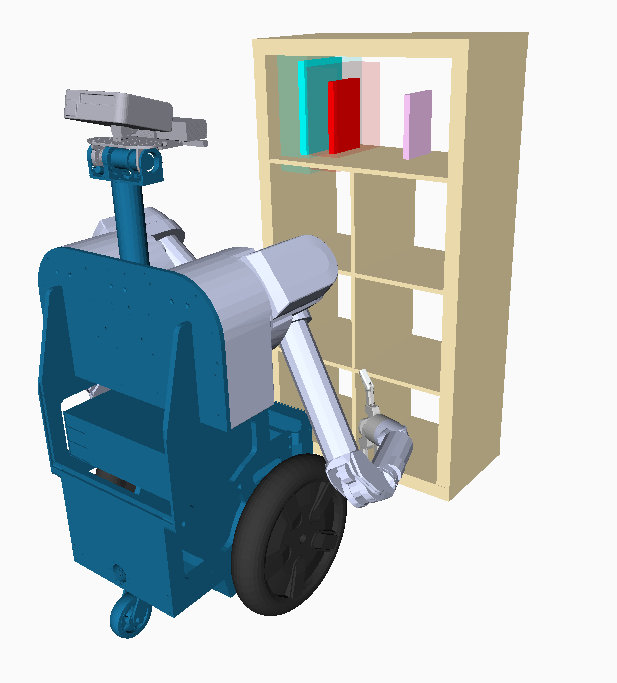
\includegraphics[width=2.6cm]{figs/herbarm-traj0-t000.png}};
      \node[inner sep=0cm] at ( 8.4,-1.45) {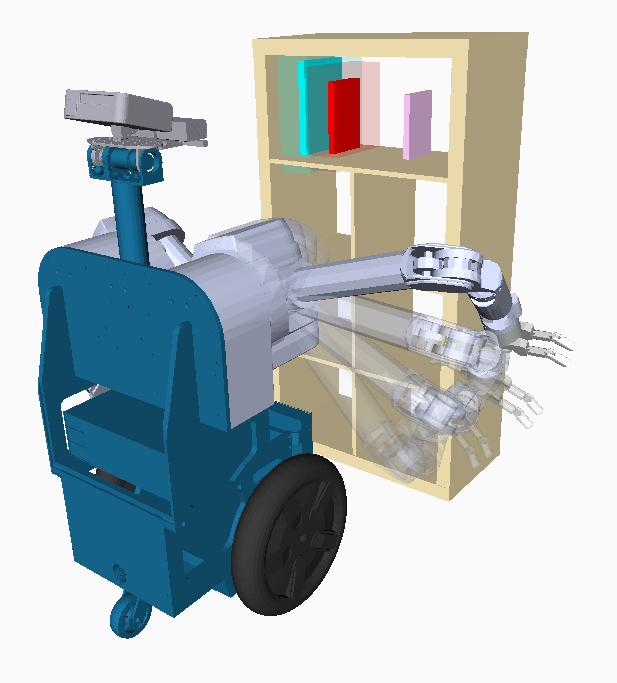
\includegraphics[width=2.6cm]{figs/herbarm-traj1-t006.png}};
      \node[inner sep=0cm] at (11.1,-1.45) {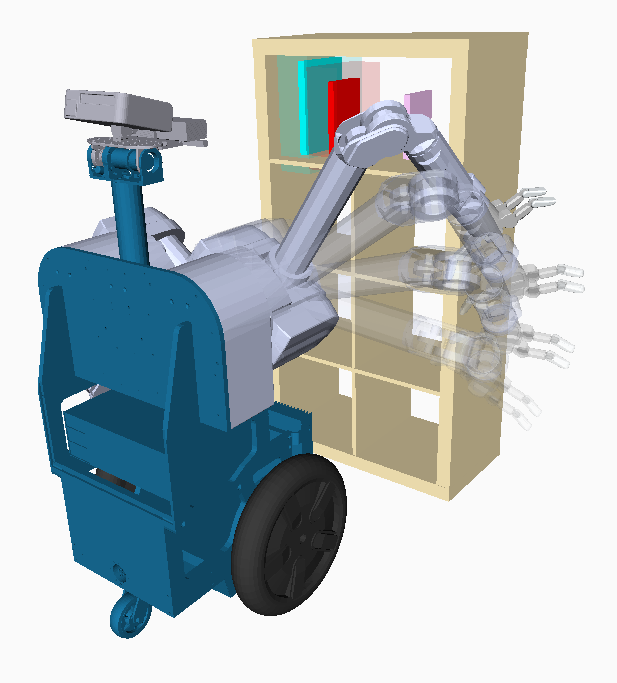
\includegraphics[width=2.6cm]{figs/herbarm-traj1-t009.png}};
      \node[inner sep=0cm] at (13.8,-1.45) {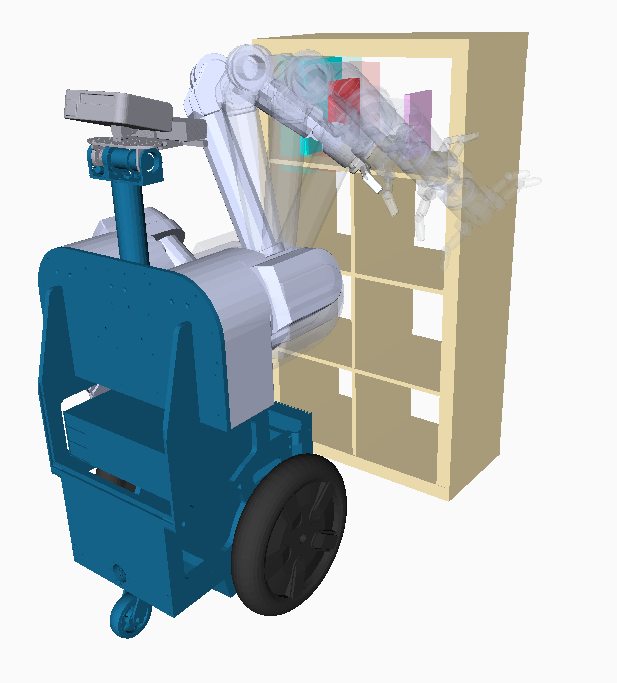
\includegraphics[width=2.6cm]{figs/herbarm-traj1-t014.png}};
      \node[inner sep=0cm] at (16.5,-1.45) {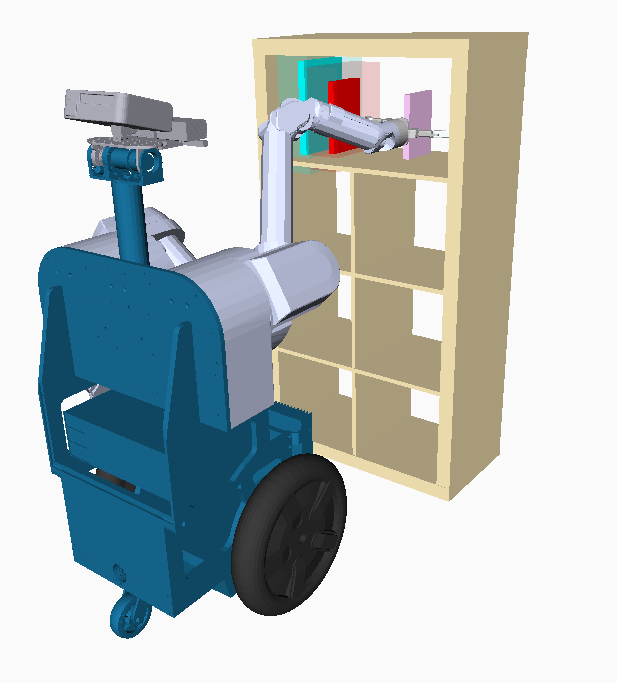
\includegraphics[width=2.6cm]{figs/herbarm-traj1-t027.png}};
      \node[fill=black!10,inner sep=0pt,minimum height=0.4cm,minimum width=3.80cm] at (3.60,-3.1) {Planning: 1.92s};
      \node[fill=black!10,inner sep=0pt,minimum height=0.4cm,minimum width=10.88cm] at (11.05,-3.1) {Execution: 5.50s};
      \node at (0.85,-2.2) {$\lambda_p = 0.5$};
      \draw[black!5] (0,0) rectangle (17.9,-3.4);
   \end{scope}
   
   % bottom row
   \begin{scope}[shift={(-1.5,-7.2)}]
      \fill[black!2] (0,0) rectangle (17.9,-3.4);
      \node[inner sep=0cm] at ( 3.0,-1.45) {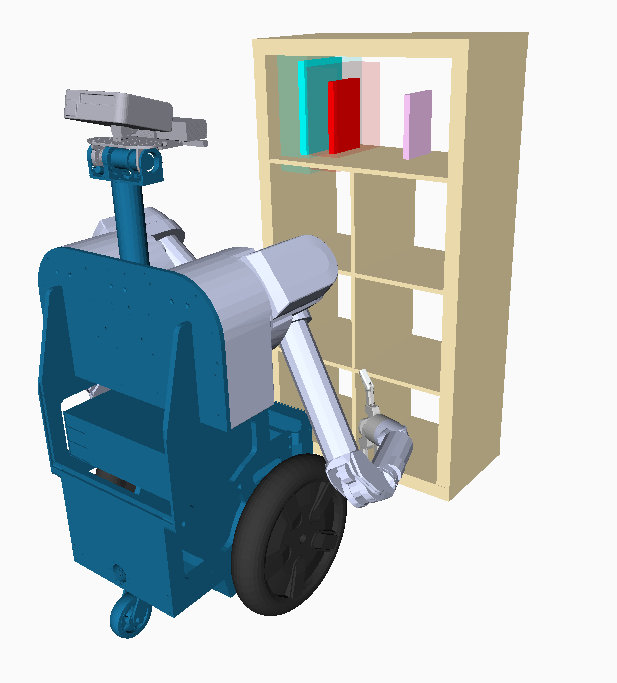
\includegraphics[width=2.6cm]{figs/herbarm-traj0-t000.png}};
      \node[inner sep=0cm] at ( 5.7,-1.45) {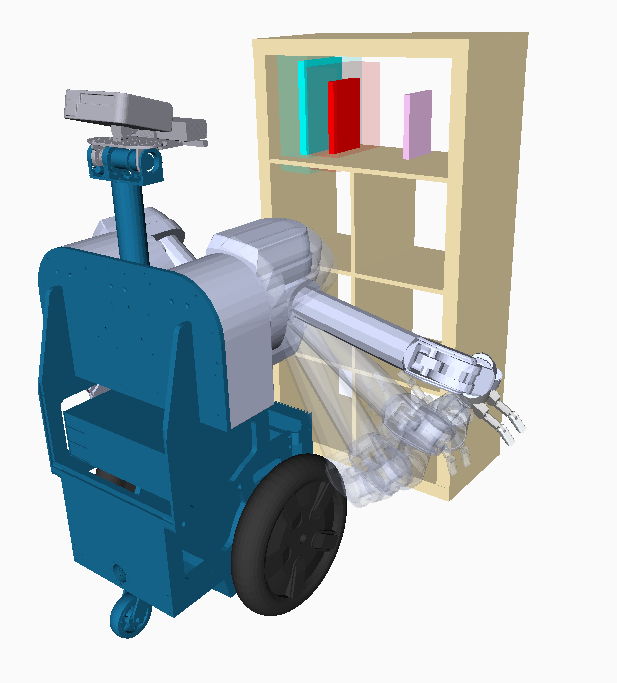
\includegraphics[width=2.6cm]{figs/herbarm-traj2-t004.png}};
      \node[inner sep=0cm] at ( 8.4,-1.45) {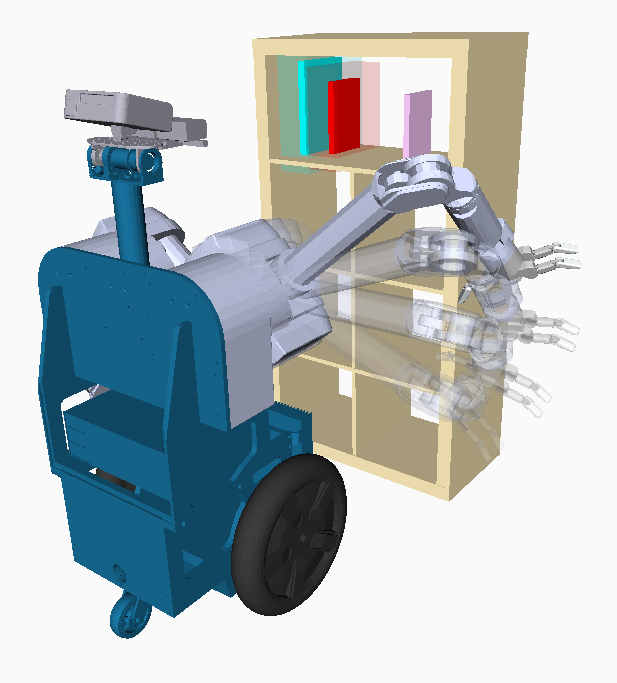
\includegraphics[width=2.6cm]{figs/herbarm-traj2-t008.png}};
      \node[inner sep=0cm] at (11.1,-1.45) {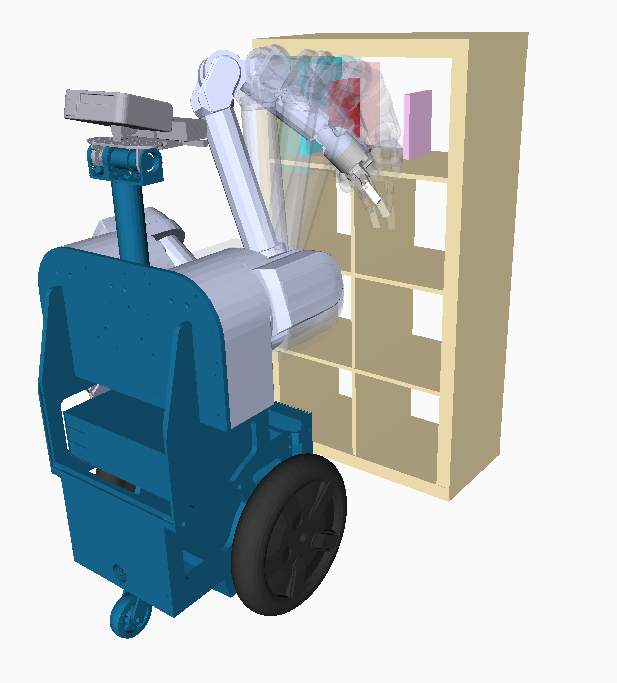
\includegraphics[width=2.6cm]{figs/herbarm-traj2-t017.png}};
      \node[inner sep=0cm] at (13.8,-1.45) {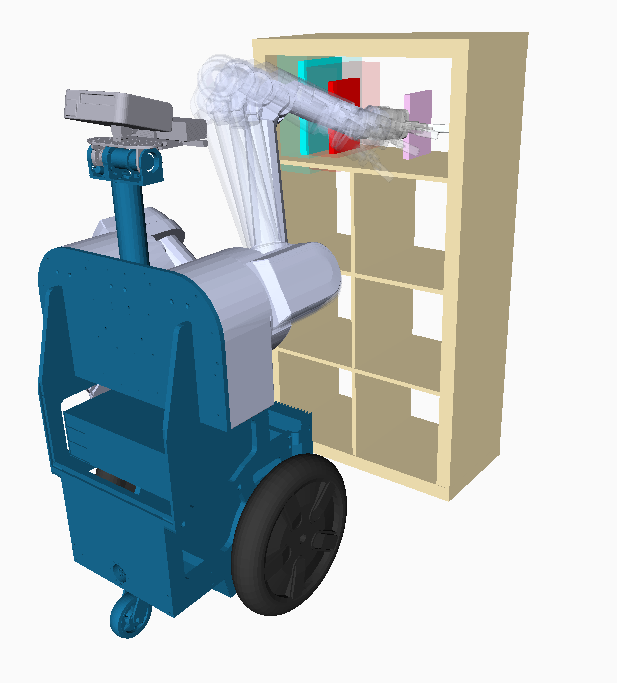
\includegraphics[width=2.6cm]{figs/herbarm-traj2-t023.png}};
      \node[inner sep=0cm] at (16.5,-1.45) {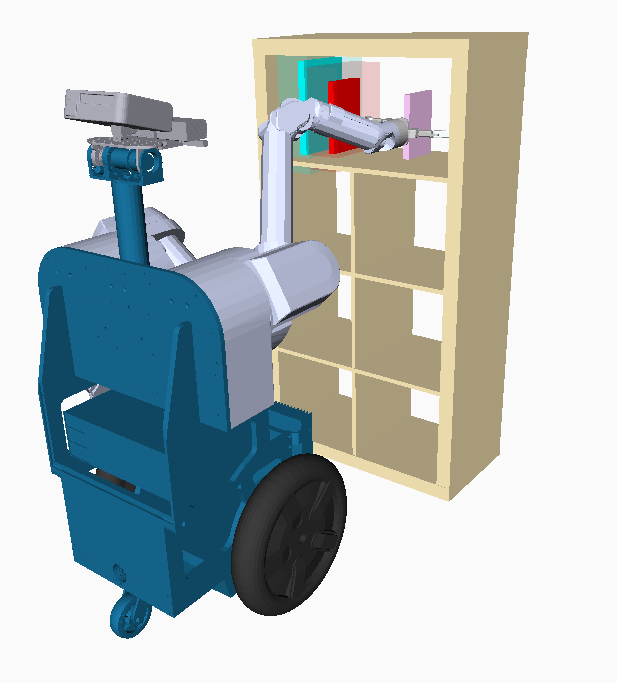
\includegraphics[width=2.6cm]{figs/herbarm-traj2-t031.png}};
      \node[fill=black!10,inner sep=0pt,minimum height=0.4cm,minimum width=2.6cm] at (3.0,-3.1) {Planning: 1.34s};
      \node[fill=black!10,inner sep=0pt,minimum height=0.4cm,minimum width=12.64cm] at (10.72,-3.1) {Execution: 6.39s};
      \node at (0.85,-2.2) {$\lambda_p = 1.0$};
      \draw[black!5] (0,0) rectangle (17.9,-3.4);
   \end{scope}

   % draw a contour on the left for each utility
   \foreach \yoffset/\rotation in {
      -1.9/0,
      -5.5/-45,
      -9.1/-90}
   {
      \begin{scope}[shift={(-1.15,\yoffset)}]
         \begin{scope}
            \clip(0,0) rectangle (1,1);
            \begin{scope}[rotate around={\rotation:(0,0)}]
               % draw simple contours
               \draw[black!60,fill=black!10] (-1,0.0) rectangle (1,1.5);
               \draw[black!60,fill=black!20] (-1,0.3) rectangle (1,1.5);
               \draw[black!60,fill=black!30] (-1,0.6) rectangle (1,1.5);
               \draw[black!60,fill=black!40] (-1,0.9) rectangle (1,1.5);
               \draw[black!60,fill=black!50] (-1,1.2) rectangle (1,1.5);
            \end{scope}
         \end{scope}
         \draw[black!60] (0,0) rectangle (1,1);
      \end{scope}
   }

\end{tikzpicture}
\end{document}
